\section{Planetas}
Los alienígenas trabajan en ayudar a la raza humana terrestre para que siga existiendo por mucho tiempo más a pesar del calentamiento global. Para ello guardan datos de los planetas del sistema solar en dos archivos de texto \texttt{planetas.txt} y \texttt{caracteristicas.txt} donde el primero tiene el formato de \texttt{planeta\#posicion}, y el segundo tiene el formato \texttt{planeta\#periodo\_rotacion\#periodo\_traslacion}.

\begin{figure}[h]
    \centering
    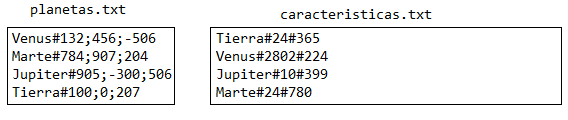
\includegraphics{Imagenes/planetas.png}
    
\end{figure}

Se le pide a usted programar las siguientes funciones
\begin{itemize}
    \item[@.] \texttt{masCercaTierra(planetas)} que reciba el nombre del archivo planetas y retorne el nombre del planeta más cercano a la tierra. Considere que la función distancia es $d=\sqrt{(x_1 -x_2)^2 + (y_1 - y_2)^2 + (z_1 - z_2)^2}$ donde $x$,$y$,$z$ son las distintas componentes de la posición.
    
    Recuerde que la tierra, al igual que otros planetas, esta en constante movimiento, por lo que la posición actual de la tierra debe ser la que el archivo \texttt{planetas} provea (no de por hecho que la tierra se encuentra en la posición del ejemplo).

\begin{lstlisting}[style=consola]
>>> masCercaTierra('planetas.txt')
'Venus'    
\end{lstlisting}
    \item[±.] \texttt{nuevo(planetas,caracteristicas)} que reciba los nombres de los archivos y escriba un nuevo archivo \texttt{galaxia.txt} con los datos fusionados de ambos archivos. Esta función no retorna nada. El formato de cada línea es \texttt{nombre\#posicion\#rotacion\#traslacion}.

\begin{figure}[h]
    \centering
    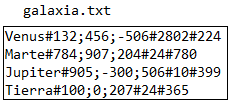
\includegraphics{Imagenes/galaxia.png}
\end{figure}
    
    \item[$\heartsuit$.] \texttt{masParecidoTierra()} que retorne el nombre del planeta cuyos tiempos de traslación y rotación sean los más parecidos con los de la tierra. Considere que la rotación de la tierra es de 24 horas y la traslación es de 365 días. La función a minimizar es $f(r,t)=(r-24)^2 + (t-365)^2$ donde $r$ y $t$ son rotación y traslación respectivamente.
    
    Esta función trabaja usando el archivo \texttt{galaxia.txt}.

\begin{lstlisting}[style=consola]
>>> masParecidoTierra()
'Jupiter'
\end{lstlisting}
\end{itemize}
